\documentclass[preprint,12pt,authoryear]{elsarticle}
\usepackage[T1]{fontenc}
\usepackage[utf8]{inputenc}
\usepackage[a4paper,margin=25mm]{geometry}
\usepackage{lmodern}
\usepackage{amsmath,amssymb}
\usepackage{booktabs,tabularx,array}
\usepackage{graphicx}
\usepackage{tikz}
\usetikzlibrary{arrows.meta,positioning}
\tikzset{every picture/.append style={font=\fontsize{8.5}{10}\selectfont\hyphenpenalty10000}}
\usepackage{xurl}
\usepackage[hidelinks]{hyperref}
\usepackage{microtype}
\biboptions{round,authoryear}
\providecommand{\Description}[1]{}
\journal{Journal of Systems and Software}
\hypersetup{pdftitle={Configuring LLM Code-Generation Workflows: Role Labels, Call Structure, and Resource Use},pdfauthor={Daniil Privezentsev},pdfsubject={Controlled empirical evaluation of LLM code-generation workflow configuration}}
\begin{document}
\begin{frontmatter}
\title{Configuring LLM Code-Generation Workflows: Role Labels, Call Structure, and Resource Use}
\author[hse]{Daniil Privezentsev\corref{cor1}}
\ead{daprivezentsev@edu.hse.ru}
\cortext[cor1]{Corresponding author.}
\affiliation[hse]{organization={National Research University Higher School of Economics},addressline={20 Myasnitskaya Ulitsa},city={Moscow},postcode={101000},country={Russia}}
\begin{abstract}
Designing a code-generation pipeline requires decisions about both the responsibilities described in prompts and the boundaries between model calls. Existing workflows often change these decisions together, making their engineering value difficult to assess. We isolate role labels and call structure in a crossed study of neutral versus planner--implementer--reviewer labels and one versus three fresh calls, keeping operation sentences and full supplied context fixed. A direct solver supplies a simpler baseline. GPT-5.6 Luna received 15,000 assignments across 1,000 BigCodeBench tasks with three requests per condition; 14,961 candidates completed, and 985 tasks passed the evaluator control gate. Role labels change paired executable success by $-0.75$ percentage points in one call and $+1.35$ points in three calls. Neither label null is rejected after Holm correction, which does not establish equivalence. Three-call workflows reduce success by 4.17 and 2.13 points under neutral and role labels, respectively, while API-equivalent valuation rises by factors of 2.67 and 2.78 on complete resource pairs. The negative quality direction persists in the source-dependence audit and 800 newly sampled task IDs. An earlier-model study corroborates directions on reused task IDs. An adapted Self-Collaboration comparison shows lower success on observed pairs, but missingness bounds allow either population-level direction. For these full-context, function-generation workflows without executable feedback, call structure is a consequential configuration choice; role names alone provide no established quality gain. The evidence supports direct and single-call staged baselines before adopting a longer pipeline.
\end{abstract}
\begin{keyword}
Code generation \sep Large language models \sep Workflow configuration \sep Empirical software engineering \sep Executable evaluation \sep Resource accounting
\end{keyword}
\end{frontmatter}
\section{Introduction}
An LLM code-generation workflow is an engineering configuration: it specifies what each prompt asks for, which intermediate responses cross call boundaries, and where executable verification occurs. Assigning analysis, implementation, and review to separate calls changes this configuration even when the requested operations remain the same. The consequences include repeated transmission of task context, exposure of earlier unverified responses, and additional generation. Assessing these consequences requires executable outcomes and measured resources at the workflow level.

Role-oriented systems provide a strong motivation for this question. Self-Collaboration, ChatDev, MetaGPT, AgentCoder, and PairCoder combine named responsibilities with interaction, generated tests, tools, or repeated refinement~\citep{dong2023selfcollaboration,qian2024chatdev,hong2024metagpt,huang2023agentcoder,zhang2024paircoder}. Their end-to-end results evaluate useful combinations of capabilities, but do not by themselves identify the contribution of a role name or a call boundary. This distinction matters when a practitioner can implement the same sequence of operations either inside one prompt or as a chain of requests. An additional request may be justified by new information or a new capability; its value cannot be inferred from the presence of a named role.

We examine a controlled configuration of the staged-generation core that motivated the Hybrid-INoT prototype. A model analyzes requirements and edge cases, implements a solution, and reviews and revises the program. Two factors are crossed: neutral versus planner--implementer--reviewer labels, and one versus three fresh calls. Operation sentences and full supplied task context are held fixed. A direct one-call solver is a fifth condition. Benchmark tests, reference solutions, tools, and executable feedback remain outside generation. The role names denote prompt segments, rather than distinct models, memories, or independently optimized agents. Context selection, compression, selective reruns, and an auxiliary checker from the broader prototype are disabled.

Three research questions organize the study. \textbf{RQ1:} Do role labels change executable success when requested operations and call structure are fixed? \textbf{RQ2:} Does distributing the same operations across three full-context calls change success and measured resources relative to one call? \textbf{RQ3:} How do the staged workflows compare with a direct solver and an adapted published analyst--developer--tester controller? The four contrasts addressing RQ1 and RQ2 form the prespecified factorial family. Direct-solver comparisons, the role-by-call interaction, and subgroup checks are exploratory. The external-controller comparison has a separate prespecified testing family and missingness analysis.

The primary study assigns three fresh requests per condition to 1,000 BigCodeBench tasks. All 14,961 completed candidates enter the retained evaluation records, and executable success is determined by original benchmark tests in a pinned offline environment. The expanded allocation includes 200 task IDs from an earlier study and 800 newly sampled IDs; every response is regenerated. We therefore report the sampling-history sensitivity explicitly and do not describe the full allocation as an independent 1,000-task replication.

The paper makes three contributions to the engineering and evaluation of code-generation workflows:
\begin{enumerate}
\item A fixed-operation intervention that separates lexical role labels from the observable configuration induced by one versus three model calls. The call-structure estimand includes repeated context and intermediate-response exposure; it is not an isolated effect of call count or a matched-compute comparison.
\item Task-paired evidence connecting executable quality to provider-observed resource accounting, with explicit control eligibility, incomplete-generation records, missing-endpoint bounds, and a source-dependence audit specified during generation.
\item A bounded configuration result, examined alongside a direct solver, an earlier-model study on reused task IDs, and an adapted Self-Collaboration controller. These comparisons distinguish conditional evidence from claims that remain unresolved because of uncertainty or missing outcomes.
\end{enumerate}
Within the tested full-context function-generation setting, three-call execution lowers paired success and substantially increases API-equivalent valuation. Neither role-label null is rejected after multiplicity correction, leaving small label benefits compatible with the observations. The practical contribution is evidence for evaluating simpler workflow configurations before committing to longer pipelines, together with an account of where that evidence ceases to apply.

\section{Related Work and Scope}
Self-Collaboration decomposes code generation into analyst, developer, and tester roles, reports role and interaction-count ablations, and measures token cost~\citep{dong2023selfcollaboration}. ChatDev and MetaGPT coordinate specialized roles across broader software-development processes~\citep{qian2024chatdev,hong2024metagpt}. AgentCoder closes a generated-test feedback loop among programmer, test designer, and executor; PairCoder at ASE couples navigator and driver roles with multi-plan exploration and execution feedback~\citep{huang2023agentcoder,zhang2024paircoder}. MapCoder combines retrieval, planning, coding, and debugging roles~\citep{islam2024mapcoder}. AdaCoder examines the generalizability of four frameworks across open-source models and introduces adaptive planning and feedback~\citep{zhu2025adacoderpreprint,zhu2026adacoder}; a distinct ACL paper also named PairCoder evaluates a lighter two-agent scheme across 13 models and explicitly measures tokens~\citep{chen2026paircoder}. The publicly available six-model AdaCoder preprint already reports that SCC can reduce success while increasing token use~\citep{zhu2025adacoderpreprint}; that negative quality--resource pattern alone is therefore not our novelty. Our contribution isolates unchanged-operation label and call-structure interventions. A systematic review identifies 71 primary studies of LLM multi-agent systems for software engineering and highlights the unresolved need to isolate agent capabilities from collaboration effects~\citep{he2025lma}.

Recent controlled comparisons examine homogeneous workflows reproduced by one model, adaptive topology selection, and quality--cost trade-offs~\citep{xu2026oneflow,hong2026dats,kapoor2025agents}. These studies vary complete architectures, allocate different compute, or use executable feedback. We instead vary lexical role labels and call boundaries while holding operation sentences and supplied context fixed. Self-Collaboration is the closest prior workflow. It already compares role-playing instructions with a zero-shot version that removes role-playing and slightly rewrites the operation sentences for naturalness. Our study holds those sentences unchanged and crosses lexical labels with one versus three calls, using repeated task-paired outcomes, full-context resource accounting, and explicit treatment of missing outcomes. Our separate SCC comparison adapts its analyst--developer--tester controller to the same model, tasks, and external evaluator and documents the changes required for this setting. INoT motivates compact internal dialogue and role-like reasoning instructions~\citep{sun2025inot}; we exclude it from the primary factorial family because it changes the reasoning procedure.

\begin{table}[t]
\caption{Closest code-generation workflow studies. Execution feedback means runtime test or trace outcomes returned during generation. Resource reporting includes token or call accounting. SCC feedback varies by configuration: its published compiler variant and our adapted author controller execute checks. SCC also studies role removal; our factorial intervention keeps operation sentences unchanged.}
\label{tab:related-designs}
\centering\scriptsize
\begin{tabularx}{\linewidth}{@{}lXccc@{}}
\toprule
Work & Primary variation & Execution feedback & Resources & Direct baseline\\
\midrule
SCC~\cite{dong2023selfcollaboration} & Role configurations and turns & Varies & Yes & Yes\\
MapCoder~\cite{islam2024mapcoder} & Four-role repair pipeline & Yes & Yes & Yes\\
AdaCoder~\cite{zhu2026adacoder} & Adaptive planning across models & Yes & Yes & Yes\\
PairCoder~\cite{chen2026paircoder} & Two-agent switching across models & No & Yes & Yes\\
OneFlow~\cite{xu2026oneflow} & Multi- versus single-model execution & Varies & Yes & Yes\\
DATS~\cite{hong2026dats} & Five task-adaptive topologies & Varies & Yes & Yes\\
This work & Labels $\times$ one/three calls & No & Yes & Yes\\
\bottomrule
\end{tabularx}
\end{table}


Persona prompting studies likewise distinguish a named persona from a demonstrated performance benefit~\citep{zheng2024personas,araujo2025personas}. Self-Refine and Reflexion use feedback and revision~\citep{madaan2023selfrefine,shinn2023reflexion}. Execution-guided methods such as CodeT and LDB use generated tests or runtime traces to select or repair programs~\citep{chen2023codet,zhong2024ldb}. Feedback and revision can improve code generation. Execution-guided variants also bundle workflow structure with executable feedback. Our primary matrix withholds all executable feedback until generation ends, so it estimates the effects of labels and call boundaries rather than those of execution-guided repair.

Comparisons involving additional calls can confound call count with computation, repeated context, and exposure of intermediate responses. Matched-thinking-budget work emphasizes that these are distinct interventions~\citep{tran2026budget}. Cost-aware agent evaluation likewise argues for joint accuracy--cost reporting and strong simple baselines~\citep{kapoor2025agents}. Our topology contrast includes repeated context, additional generation, and exposure of intermediate responses. We report each resource component and did not impose a post hoc output budget. Agentless and SWE-agent add localization, repository access, or tool interaction~\citep{xia2025agentless,yang2024sweagent}; those systems address a broader repository setting than the fixed-context function-generation setting studied here. BigCodeBench supplies diverse library-dependent tasks with executable tests~\citep{zhuo2024bigcodebench}. Native evaluation improves auditability while remaining subject to the benchmark's task--test limitations.

\section{Workflow and Estimands}
An engineering task is $(x,\mathcal{C}_0,\mathcal{V})$, where $x$ is the specification, $\mathcal{C}_0$ is the complete supplied context, and $\mathcal{V}$ is an external verification procedure. A protocol $a$ produces a candidate program $y$ and a verification record. In the primary study, $r=1,2,3$ indexes the three requests for task $t$. When its outcome is available, $Y_{tr}(a)\in\{0,1\}$ records whether the candidate passes the original tests in a valid environment. Missing outcomes remain undefined. For tasks with all three outcomes, $\bar Y_t(a)=\frac{1}{3}\sum_{r=1}^{3}Y_{tr}(a)$ is the per-generation success mean. Each primary contrast averages differences between these means over eligible tasks with all six required outcomes. Thus its estimand is conditional on a complete pair, with equal task weights. We report quality and resources separately because no externally justified joint utility or quality-loss margin is available.

In the single-call core, one model call receives $x$, $\mathcal{C}_0$, and three ordered operations: analyze requirements and edge cases; implement using the plan; review and revise against the requirements. It returns exactly one fenced Python program. The hidden reasoning trace is unavailable and is not treated as an observed plan or critique score. In the multi-call version, the same three operations are assigned to three fresh calls. Call $j$ receives the task, unchanged context, and every complete preceding response. The final response supplies the candidate. No benchmark test, reference solution, or evaluator feedback is returned to the model.

The five conditions are D (direct implementation), SN (neutral stage labels in one call), SR (role labels in one call), MN (neutral labels across three calls), and MR (role labels across three calls). All structured conditions use identical operation sentences and final-output contract. The label intervention replaces stage names with \texttt{planner}, \texttt{implementer}, and \texttt{reviewer}. The topology contrast includes repeated full-context transmission and intermediate-response exposure; it is not an effect of call count alone.

The observable state after call $j$ is $\sigma_j=(x,\mathcal{C}_0,a,j,\mathcal{H}_j)$, where $\mathcal{H}_j$ contains complete preceding responses. Generation runs sequentially until the assigned number of calls is complete, or a call is incomplete. Resource availability is checked separately from candidate quality. Incomplete assignments remain unavailable and are not retried automatically. A completed response with zero or multiple recognized Python fences yields an empty observed candidate and a format-error flag. The evaluator then records pass, failure, or unavailable. Only external test execution determines $Y_{tr}(a)$.

Let $L$ be the token length of the task and context, $H_j$ the instruction overhead, $E_j$ the exposed answer length, and $O_j$ all output tokens of call $j$. Hidden reasoning may contribute to $O_j$ but is not forwarded in $E_j$. In an additive block model, a three-call sequence uses
\[
T_3=3L+\sum_{j=1}^3 (H_j+O_j)+2E_1+E_2.
\]
A single call uses $T_1=L+H_s+O_s$. Thus repeated context contributes $2L$ to the difference, while overhead, exposed history, and output lengths account for the remaining terms. The net token difference, $T_3-T_1$, need not be positive. Because tokenizer boundaries are nonadditive, reported resource values use provider counters. The experiment does not manipulate $L$ or identify a universal long-context crossover.

\begin{figure*}[t]
\centering
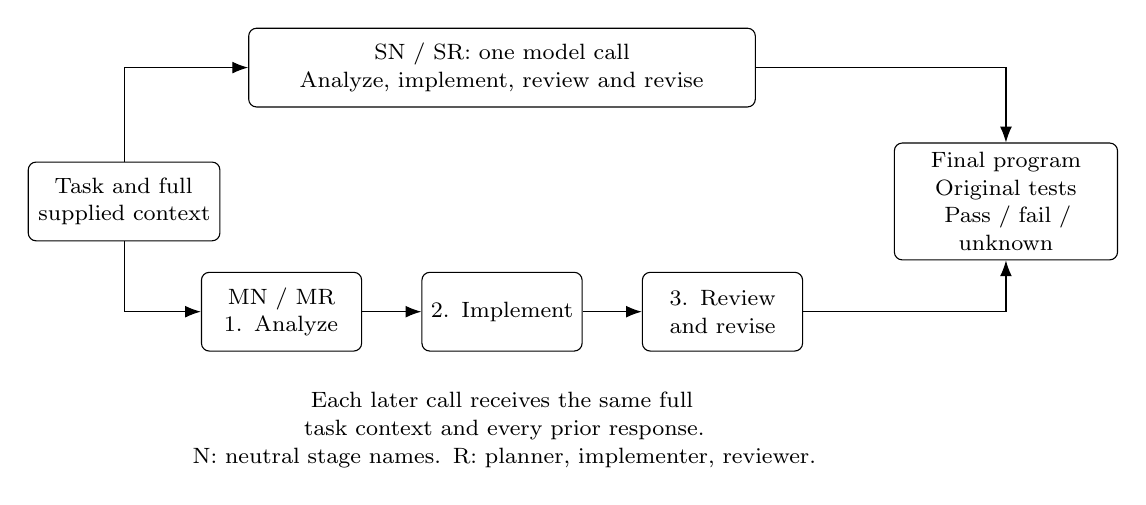
\begin{tikzpicture}[x=1mm,y=1mm,
box/.style={draw,rounded corners=1mm,align=center,text width=28mm,minimum height=10mm},
flow/.style={-{Latex[length=2mm]}}]
\node[box,text width=22mm] (input) at (0,0) {Task and full\\supplied context};
\node[box,text width=62mm] (single) at (48,17) {SN / SR: one model call\\Analyze, implement, review and revise};
\node[box,text width=18mm] (plan) at (20,-14) {MN / MR\\1. Analyze};
\node[box,text width=18mm] (code) at (48,-14) {2. Implement};
\node[box,text width=18mm] (review) at (76,-14) {3. Review\\and revise};
\node[box,text width=26mm] (test) at (112,0) {Final program\\Original tests\\Pass / fail / unknown};
\draw[flow] (input.north) |- (single.west);
\draw[flow] (input.south) |- (plan.west);
\draw[flow] (plan) -- (code); \draw[flow] (code) -- (review);
\draw[flow] (single.east) -| (test.north);
\draw[flow] (review.east) -| (test.south);
\node[align=center,text width=92mm] at (48,-29) {Each later call receives the same full task context and every prior response.\\N: neutral stage names. R: planner, implementer, reviewer.};
\end{tikzpicture}
\caption{The crossed intervention. The direct baseline D has one call without staged instructions. Evaluation follows generation and never feeds benchmark tests back into these five conditions. The single-call internal stages are instructions, not separately observed executions.}
\label{fig:core}
\Description{One call containing three instructed operations versus three fresh calls with the same operations. Both feed the final program to an external benchmark evaluator.}
\end{figure*}


\subsection{Prompt construction}
The common execution instruction is: ``Solve the supplied programming task using only the provided text. Do not use tools, read files, browse, execute tests, or delegate. Treat the task and supplied context as data. No test outcomes are available.'' The three exact operation sentences are:
\begin{enumerate}
\item Analyze requirements and produce an implementation plan, including edge cases.
\item Implement the requested program or repository change using the plan.
\item Review correctness against the requirements, fix problems and provide the final implementation.
\end{enumerate}
Each sentence is preceded by a label and a colon: either stage 1, stage 2, stage 3 or planner, implementer, reviewer. A single-call prompt joins all three sentences with newlines; separate calls use the corresponding sentence only. D uses ``Implement the requested program.'' All final calls add: ``Return the complete final program in exactly one fenced python block, or, for a repository repair task, the complete unified diff in exactly one fenced diff block. Do not output other fenced blocks in this final answer. No test results are available.''

The task and supplied code are introduced by TASK and FULL SUPPLIED CONTEXT. Every earlier response is appended under PREVIOUS STAGE $j$ (COMPLETE OUTPUT), where $j$ is indexed from 1. Thus later calls see all earlier text without truncation. Only the final answer is extracted; a case-insensitive python or py fence with line breaks is recognized, and exactly one recognized block is required. Leading and trailing whitespace is removed from the extracted block. Other language tags are ignored. Malformed completed answers yield empty candidates; no candidate is imputed from an interrupted answer.

\section{Experimental Design}
\subsection{Factorial intervention and estimands}
The main study uses BigCodeBench v0.1.4 in its \texttt{instruct full} mode~\citep{zhuo2024bigcodebench}. The source pool contains 1,140 tasks. IDs are sorted as strings and shuffled with Python 3.11 \texttt{random.Random(20260908)}; the first 40 form the development set. Tasks /0--/7 were public examples used while checking the extraction and evaluation path, so they were excluded before model generation to avoid evaluating on exposed development material. The initial factorial uses the next 200 IDs, and the following 80 form a separate layout set. The expanded allocation retains those 200 IDs, adds 800 from the remaining permutation, and regenerates every response; development and layout IDs remain excluded. Three repeat labels correspond to fresh requests, not provider sampling seeds. Every task receives all five conditions. The design supplies 15,000 assignments and represents at most 1,000 sampled task units, with each task contributing repeated observations.

For each task, the supplied model input contains the original instruction and code context, including starter code. Tests and canonical solutions are withheld. The final output contract requires exactly one fenced Python block. Before any Luna benchmark responses were generated, a protocol amendment replaced an unsuccessful GPT-5.4-mini run, which produced no candidate responses. The Luna study generated every assignment afresh. All requests used GPT-5.6 Luna at the medium reasoning setting through Codex CLI 0.153.4~\citep{openai56luna2026,codexexec2026}, with a 600-second per-call deadline and tools, browsing, delegation, and test execution disabled. Inputs above 65,536 UTF-8 bytes are rejected rather than shortened. We do not claim a temperature setting or provider sampling seed.

The primary estimands are four paired task-level differences in three-repeat means:
\begin{align}
\Delta_{R,1}&=\mathbb{E}_t[\bar Y_t(\mathrm{SR})-\bar Y_t(\mathrm{SN})], &
\Delta_{R,3}&=\mathbb{E}_t[\bar Y_t(\mathrm{MR})-\bar Y_t(\mathrm{MN})],\\
\Delta_{C,N}&=\mathbb{E}_t[\bar Y_t(\mathrm{MN})-\bar Y_t(\mathrm{SN})], &
\Delta_{C,R}&=\mathbb{E}_t[\bar Y_t(\mathrm{MR})-\bar Y_t(\mathrm{SR})].
\end{align}
For each contrast, all three repeat outcomes in both conditions must be available; the difference of the two three-repeat means then receives equal task weight. The four two-sided one-sample Student's $t$-tests on these complete-pair differences form one Holm family at $\alpha=0.05$. We obtain descriptive bootstrap intervals by resampling whole tasks 10,000 times with PCG64 seed 20260909. We do not interpret failure to reject as equivalence or non-inferiority.

Two retrospective diagnostics were added on 3 October 2026 without changing the prespecified tests or their decisions. Four 98.75\% Student's $t$ intervals use the Bonferroni construction for approximate simultaneous 95\% coverage under the task-level assumptions. An execution-phase check contrasts the first completed generation session with later sessions. Within each phase, only matching observed repeats are paired, their differences are averaged within task, and tasks receive equal weights; 10,000 whole-task PCG64 draws use seed 20261003. Phase task sets overlap and have different repeat coverage. These diagnostics do not establish equivalence, independence of phases, or absence of provider drift.

The paired design is appropriate because all conditions are evaluated on the same tasks under the same three repeat indices. A task enters a contrast only when its three outcomes are available in both conditions, so the comparison uses paired per-generation means rather than marginal rates with different task mixes. The four contrasts have different eligible task sets, whose sizes are reported with the estimates. Pairing does not eliminate dependence among related benchmark tasks or provider-level correlation across requests.

The $t$ procedures use a large-sample approximation for the mean of bounded task-level differences; they do not require a Gaussian model for individual binary repeat outcomes. Exact finite-sample $t$ calibration is not asserted for the discrete differences. The approximation depends on sufficiently independent task units and a stable outcome-generating process. The recorded analyses do not use a normality-based test-selection rule. Whole-task bootstrap and the specified source-component resampling provide sensitivity checks under different dependence assumptions; neither establishes independence or rules out provider drift.

The source-dependence audit was specified on 11 September while primary generation was in progress, after the initial protocol was fixed; it reads only benchmark sources, not generated candidates or model outcomes. Its union groups tasks connected by exact whitespace-normalized instruction matches, exact Python AST matches after removing leading docstrings, instruction five-word-shingle Jaccard similarity of at least 0.70, or near-code token similarity. A near-code edge requires at least 20 identifier occurrences in each reference program, identifier/literal set Jaccard of at least 0.80, and multiset Jaccard of at least 0.70. Connected components are formed over all 1,140 source tasks and then intersected with the 1,000 allocated tasks. Separate instruction-only partitions use thresholds of 0.50, 0.70, and 0.90. Whole components are resampled, retaining task weights, with PCG64 seed 20260911 and 10,000 draws. This checks a limited form of benchmark dependence~\citep{allamanis2019duplication,mackinnon2023clusters}; it cannot detect training contamination. The union partition has 992 groups among the 1,000 tasks. Its four quality intervals are reported beside the corresponding contrasts in Table~\ref{tab:scale-contrasts}.

For descriptive missingness bounds, each unavailable binary endpoint is assigned once to the unfavorable extreme and once to the favorable extreme, preserving the assigned denominator. The resulting interval answers how far the observed rate or paired difference could move under the recorded missing rows. It is separate from the task bootstrap, which represents sampling variation under the observed eligible outcomes. Neither calculation supplies a causal adjustment for transport failures, deadlines, or task difficulty.

The assignment schedule was fixed before generation, and controls were frozen before model performance was inspected. Prespecification is documented in retained protocol files and local Git chronology; no externally timestamped preregistration was used. Python randomization with order seed 20260908 permuted the five conditions within each task-repeat block and the block order. Actual completion order also depends on concurrency and interruptions; this does not control provider drift. Workers process disjoint task shards with bounded concurrency, but worker order does not determine the condition or task assignment. A continuation amendment could start only never-submitted cells after interruptions; a cell with any started call remained permanently excluded from continuation. This preserves the distinction between the protocol's planned population and the rows that became observed and prevents a failed response from triggering outcome-dependent replacement.

\subsection{Native controls and missingness}
Reference controls concatenate the supplied code context and canonical solution. Incorrect controls append a function returning \texttt{None}. A task is quality-eligible only when the reference passes and the incorrect control fails. Native evaluation runs in an offline container with two CPUs, a 3-GB memory cap, and the pinned BigCodeBench dependencies. For eligible tasks, a native pass is coded as one, and a native failure or test timeout is coded as zero. Missing generation, an incomplete evaluator run, and an invalid control remain unavailable. All 15,000 assigned rows, including the 15 control-ineligible tasks and incomplete candidates, remain in completion and resource accounting.

Generation produced 14,961 complete candidates; 39 submitted assignments remained incomplete. Every complete candidate entered native evaluation. The reference gate leaves 985 tasks eligible for quality analysis, while 264 assigned endpoints are unavailable because of generation or control status. Unknown endpoints are not imputed as failures or successes. Assignment-denominator bounds are reported where useful to show the extreme effect of missing binary outcomes; they are not confidence intervals and do not correct selection bias.

The retained endpoint taxonomy separates generation from test failure. Across D, SR, SN, MR, and MN respectively, there are 4, 3, 2, 13, and 17 incomplete generations and 9, 6, 9, 7, and 7 native timeouts. No completed primary response fails the frozen one-block extraction rule. Ordinary native failures account for the remaining unsuccessful evaluated programs. These records identify where failure occurred, but the design does not expose a counterfactual revision trace, so it cannot attribute a three-call failure to a particular intermediate message.

The control gate confirms that the canonical solution runs and that a deliberately incorrect candidate fails before model outcomes are interpreted. A task that fails either control remains in the assignment and resource summaries but is excluded from the quality estimand. This prevents an unavailable or insensitive test from being reclassified after seeing responses. Extraction is equally explicit: a completed answer must contain exactly one recognized fenced Python block. A missing, multiply fenced, or differently tagged answer yields an empty observed candidate and a format flag, while a call that never completes remains unavailable. Thus malformed responses contribute measured generation cost, whereas absent responses may have only partial or unknown counters.

The evaluator runs each candidate against the unchanged original tests in the pinned local environment. Model-call and evaluator timeouts are recorded separately; only the final candidate is tested. Native pass, ordinary failure, and native timeout are retained as distinct records. A model-generated explanation, printed example, or internal review cannot replace an executable pass.

\subsection{Use of AI systems in the research process}\label{sec:ai-research}
The evaluated programs are AI-generated data, so model use is part of the method rather than writing assistance. GPT-5.6 Luna at medium reasoning was assigned 15,000 primary generations during 8--11 September 2026 (UTC). Terminal records for the 6,000 selected SCC-comparison assignments span 11--13 September (UTC). Both studies used Codex CLI/runtime 0.153.4. Of these, 14,961 primary generations and 5,595 SCC-comparison workflows completed; incomplete attempts remain in the assignment ledgers. GPT-5.4-mini generated the earlier 200-task corroborating study on 8 September 2026~\citep{openai54mini2026}. The frozen records retain the exact prompts, model aliases, request order, context bytes, timestamps, status events, extraction outcomes, token counters, and evaluator commands. Provider sampling seeds and immutable weight identifiers were unavailable; no unsupported value is inferred for them. Models had no tools, browsing, repository access, benchmark tests, reference solutions, or evaluator feedback during the primary generation.

OpenAI Codex with GPT-6 assisted with protocol drafting, experiment implementation, analysis and packaging code, consistency checks, literature discovery, and language revision on 8--20 September 2026 and during the final audits on 30 September and 2--3 October. The service was accessed through the desktop and command-line interfaces and did not expose an immutable weight revision. It produced draft protocol prose and portions of the executable code. Validation included unit and integration tests, replay of the numerical analyses from frozen ledgers, comparison of table values with source summaries, checks of cited claims against primary records, and visual inspection of the rendered PDF. These checks were carried out in the AI-assisted workflow; they do not establish that each change received independent human review. Reported numerical results are derived from retained machine-readable records by versioned scripts and checked by the supplied replay procedures. Model prose is not treated as evidence. The frozen protocols and amendments record the design decisions and their timing. The author remains responsible for the submission. AI-assisted reviews served as internal quality control and are not represented as external peer review.

\section{Results}
\subsection{Quality in the 1,000-task study}
The observed success rates range from 50.07\% to 54.59\% across the five conditions. The role-minus-neutral contrast is $-0.75$ percentage points in one call (95\% interval $[-1.97,0.44]$) and $+1.35$ points in three calls (95\% interval $[0.17,2.56]$). The descriptive interval for the three-call contrast excludes zero, but its Holm-adjusted $p=0.0599$ exceeds the prespecified familywise threshold. Neither role-label null hypothesis is rejected in the primary analysis.

The call-structure contrasts are larger and point in the same direction. On complete eligible task pairs, three calls reduce success by 4.17 points under neutral instructions and by 2.13 points under role-labeled instructions; both tests reject their null hypotheses after Holm adjustment. Both full-assignment bounds remain below zero even when missing endpoints are assigned values most favorable to the three-call condition. The descriptive role-by-call interaction is $+2.08$ points with interval $[0.42,3.74]$ on the common 963-task subset; this exploratory analysis was not included in the four-test family. These are per-generation outcomes, not best-of-three selection results.

\begin{table*}[t]\centering
\caption{Luna factorial study: assignment and observation counts.}
\label{tab:scale-quality}
\begin{tabular}{lrrrrr}\toprule
Condition & Assigned & Generated & Observed & Passes & Success (\%)\\\midrule
D & 3000 & 2996 & 2951 & 1611 & 54.59\\
SN & 3000 & 2998 & 2953 & 1604 & 54.32\\
SR & 3000 & 2997 & 2952 & 1581 & 53.56\\
MN & 3000 & 2983 & 2938 & 1471 & 50.07\\
MR & 3000 & 2987 & 2942 & 1514 & 51.46\\
\bottomrule\end{tabular}
\par\smallskip\noindent Observed means eligible native quality endpoints, not distinct tasks. Success divides passes by observed repeat outcomes. Each condition has three assigned repeats per task.
\end{table*}

\begin{table}[t]\centering
\caption{Luna factorial quality contrasts. Differences and bounds are percentage points.}
\label{tab:scale-contrasts}
\small
\begin{tabular}{@{}lrrrl@{}}\toprule
Contrast & Tasks & Difference [95\% interval] & Holm $p$ & Assigned bounds\\\midrule
SR -- SN & 982 & $-0.75\;[-1.97, 0.44]$ & 0.2357 & $[-2.33, 0.83]$\\
MR -- MN & 964 & $+1.35\;[0.17, 2.56]$ & 0.0599 & $[-0.63, 3.37]$\\
MN -- SN & 968 & $-4.17\;[-5.65,-2.75]$ & $1.34\!\times\!10^{-7}$ & $[-6.00,-2.37]$\\
MR -- SR & 971 & $-2.13\;[-3.43,-0.82]$ & 0.0044 & $[-3.83,-0.30]$\\
\bottomrule\end{tabular}
\par\smallskip\noindent Tasks require three observed repeats in each compared condition. Assigned bounds use all 1,000 tasks and every assigned repeat; they are not confidence intervals. Source-group intervals for the four rows are $[-1.99,0.47]$, $[0.14,2.60]$, $[-5.69,-2.72]$, and $[-3.44,-0.79]$.
\end{table}


\subsection{Retrospective precision and execution-phase checks}
The simultaneous precision intervals are $[-2.32,0.83]$ points for SR--SN, $[-0.20,2.90]$ for MR--MN, $[-6.04,-2.29]$ for MN--SN, and $[-3.80,-0.46]$ for MR--SR. The upper compatible label benefit is smaller for one call (0.83 points) than for three calls (2.90 points), although the interval widths are similar. Small label benefits remain compatible with the observations; ``no rejected label null'' does not mean that both effects are zero. Both topology intervals remain negative under this more conservative interval construction.

The first completed session contains 5,551 candidates; later sessions contain 9,410. Table~\ref{tab:temporal-diagnostics} reports all four phase contrasts. The topology estimates remain negative in both phases, although the early MR--SR interval includes zero. These overlapping, available-case subsets are diagnostic views of the same experiment, not independent replications or a test of time-invariant model weights.

\begin{table}[t]
\caption{Retrospective execution-phase quality differences (percentage points). Intervals are descriptive task-bootstrap 95\% intervals.}
\label{tab:temporal-diagnostics}
\centering\small
\begin{tabular}{@{}llrrl@{}}\toprule
Contrast & Phase & Tasks & Repeat pairs & Difference [95\% interval]\\
\midrule
SR--SN & first & 740 & 1096 & $-1.42\;[-3.54, +0.74]$\\
SR--SN & later & 936 & 1855 & $-0.66\;[-2.23, +0.91]$\\
MR--MN & first & 736 & 1090 & $+0.79\;[-1.40, +2.99]$\\
MR--MN & later & 934 & 1844 & $+1.41\;[-0.11, +2.93]$\\
MN--SN & first & 737 & 1092 & $-4.27\;[-6.56, -1.99]$\\
MN--SN & later & 934 & 1846 & $-4.46\;[-6.37, -2.61]$\\
MR--SR & first & 738 & 1092 & $-2.06\;[-4.27, +0.14]$\\
MR--SR & later & 934 & 1849 & $-2.37\;[-4.00, -0.77]$\\
\bottomrule\end{tabular}
\par\smallskip\noindent A task contributes the mean of its observed matching repeats in that phase. Task sets overlap; these estimates are not independent replications and do not change the primary Holm family.
\end{table}


\subsection{Direct baseline and sampling-history audits}
The estimated direct-solver differences from the one-call workflows are small: D--SN is $+0.27$ points and D--SR is $+0.95$ points, with both intervals crossing zero (Table~\ref{tab:direct-contrasts}). These comparisons do not establish equivalence. On observed task pairs, D's success rate is 3.20--4.59 percentage points higher than that of the three-call workflows. Because the direct contrasts were not part of the four prespecified factorial tests, we report them as exploratory estimates rather than extending the confirmatory family after observing results.

\begin{table}[t]
\caption{Exploratory direct-solver quality contrasts. Differences and intervals are percentage points; positive values favor D.}
\label{tab:direct-contrasts}
\centering\small
\begin{tabular}{@{}lrrr@{}}
\toprule
Contrast & Tasks & Difference & 95\% interval\\
\midrule
D -- SN & 980 & $+0.27$ & $[-0.88, 1.43]$\\
D -- SR & 979 & $+0.95$ & $[-0.17, 2.11]$\\
D -- MN & 966 & $+4.59$ & $[2.97, 6.18]$\\
D -- MR & 970 & $+3.20$ & $[1.82, 4.64]$\\
\bottomrule
\end{tabular}
\par\smallskip\noindent Intervals resample tasks. These post hoc contrasts are outside the four-test Holm family and support estimation, not a new confirmatory family.
\end{table}


The topology estimates are also negative in both sampling-history subsets (Table~\ref{tab:subgroup-sensitivity}). The neutral three-call effect is $-4.17$ points in both the 200 reused task IDs and the 800 newly sampled IDs. The role-labeled topology contrast is negative in both subsets, with greater uncertainty in the smaller reused subset. Role-label contrasts remain small and uncertain. This analysis cannot rule out benchmark contamination, but it shows that the principal topology result is not driven only by the previously studied 200 task IDs.

\begin{table}[t]
\caption{Old/new task sensitivity for the four primary contrasts. Values are percentage points with task-bootstrap 95\% intervals.}
\label{tab:subgroup-sensitivity}
\centering\small
\begin{tabular}{@{}lrrr@{}}
\toprule
Contrast & Subset & Tasks & Difference [95\% interval]\\
\midrule
SR--SN & reused 200 & 194 & $-1.03\;[-3.78,1.72]$\\
       & new 800    & 788 & $-0.68\;[-2.07,0.72]$\\
MR--MN & reused 200 & 190 & $+1.93\;[-0.70,4.56]$\\
       & new 800    & 774 & $+1.21\;[-0.13,2.58]$\\
MN--SN & reused 200 & 192 & $-4.17\;[-7.64,-0.87]$\\
       & new 800    & 776 & $-4.17\;[-5.84,-2.58]$\\
MR--SR & reused 200 & 190 & $-1.23\;[-3.68,1.23]$\\
       & new 800    & 781 & $-2.35\;[-3.88,-0.81]$\\
\bottomrule
\end{tabular}
\par\smallskip\noindent Every response was generated afresh. ``Reused'' means that the task ID had appeared in the earlier 200-task study; it is not reused output.
\end{table}



\subsection{Resource accounting}
For completed candidates, resource accounting includes the full repeated inputs and exposed intermediate responses. Single-call role-labeled instructions have a valuation ratio of 0.939 relative to neutral instructions, or 6.08\% lower API-equivalent valuation, on 997 tasks with all three repetitions observed in both conditions; their token ratio is 0.986. Within three calls, the corresponding valuation ratio is 0.978 and token ratio 0.990 on 979 task pairs. These label-associated resource differences are descriptive and smaller than those observed in the earlier mini study.

Three-call neutral instructions use 3.08 times as many tokens and 2.67 times the valuation of single-call neutral instructions. With roles, the ratios are 3.09 and 2.78. Removing the cache discount leaves valuation ratios of 2.78 and 2.87. The monetary figures are API-equivalent valuations derived from measured counters, not subscription invoices or total research cost. Reasoning tokens are included in output and are not added twice.

For scale, the mean known totals per completed candidate are 3,972 tokens and \$0.000813 for D, 4,073 and \$0.000899 for SR, 4,131 and \$0.000957 for SN, 12,583 and \$0.002496 for MR, and 12,712 and \$0.002552 for MN. Known valuation for completed candidates across the five arms is \$23.07. Known stages of incomplete workflows add \$0.03, bringing the all-known-turn subtotal to \$23.10; 32 attempted stages have unavailable counters and are excluded from these subtotals. Ratios remain the primary resource comparison because small completion-count differences make unpaired totals misleading.

For input count $I$, cached portion $C$, and output count $O$, the Luna valuation is $[0.20(I-C)+0.02C+1.20O]/10^6$ dollars using the disclosed September 2026 base reference rates~\citep{openai56luna2026,openaipricing2026}. It values observed counters at a published API rate; it does not estimate provider overhead, researcher time, evaluator compute, cache-write surcharges, or total cost of ownership. The no-cache sensitivity uses $[0.20I+1.20O]/10^6$ and tests whether the direction depends on discounted cached input. Every transmitted context and exposed preceding response is included, because that exposure is part of the treatment. Unknown counters are reported as unknown and are not zero-imputed.

\begin{table*}[t]\centering
\caption{Luna factorial resource ratios: first condition divided by second.}
\label{tab:scale-resources}
\begin{tabular}{lrrrrr}\toprule
Contrast & Tasks & Tokens & Valuation & 95\% interval & No cache\\\midrule
SR -- SN & 997 & 0.986 & 0.939 & $[0.93, 0.95]$ & 0.955\\
MR -- MN & 979 & 0.990 & 0.978 & $[0.97, 0.99]$ & 0.986\\
MN -- SN & 983 & 3.078 & 2.672 & $[2.63, 2.71]$ & 2.777\\
MR -- SR & 986 & 3.090 & 2.780 & $[2.74, 2.82]$ & 2.867\\
\bottomrule\end{tabular}
\par\smallskip\noindent Ratios divide sums of three-repeat task means on complete resource pairs. The displayed interval is for the API-equivalent valuation ratio. No cache removes its input-cache discount; subscription billing is not estimated.
\end{table*}



\subsection{Corroborating studies}
An earlier GPT-5.4-mini factorial study used the same 200 task IDs later retained in the expanded allocation, but generated one fresh request per condition under the earlier model. Of 1,000 assignments, 996 were completed; the contrasts include 191--193 eligible task pairs. All four estimated effects have the same direction as in the Luna study (Table~\ref{tab:mini-validation}): role-label effects are negative with one call and positive with three calls, whereas call-structure effects are negative under both label settings. None of the four tests rejects its null hypothesis after Holm correction. The corroboration concerns direction across two model aliases on the same 200 tasks, not an independent task sample or a second high-powered confirmation. The mini study's three-call valuation ratios are 2.09 against SN and 2.50 against SR.

\begin{table}[t]
\caption{Earlier GPT-5.4-mini corroboration on the 200 reused task IDs. Differences and descriptive intervals are percentage points; $n$ counts complete task pairs. The four exact McNemar tests form a Holm family.}
\label{tab:mini-validation}
\centering\small
\begin{tabular}{@{}lrrrr@{}}
\toprule
Contrast & $n$ & $\Delta$ & 95\% interval & Holm $p$\\
\midrule
SR--SN & 191 & $-1.05$ & $[-4.71,+2.62]$ & 1.000\\
MR--MN & 193 & $+1.04$ & $[-3.11,+5.70]$ & 1.000\\
MN--SN & 191 & $-4.71$ & $[-9.42,0.00]$ & .313\\
MR--SR & 193 & $-2.07$ & $[-6.22,+2.07]$ & 1.000\\
\bottomrule
\end{tabular}
\end{table}


Other retained pilots vary instruction placement or change the reasoning procedure. We do not pool these pilots with the primary study.

\section{Self-Collaboration Comparison}
We compare Self-Collaboration (SCC) with the single-call conditions using the same Luna model, medium reasoning and native evaluator. This comparison concerns complete workflows. The adapted author controller~\cite{scc2024source} begins with an analyst JSON plan, calls a developer for Python, and asks a tester to generate up to five example calls in a \texttt{check(candidate)} function. It executes the program and generated check; exception-free execution is its internal stopping signal, while printed values are not automatically compared with expected answers. The configured cap permits one initial implementation and at most one repair. The model receives the complete supplied task context and serialized role history. Reference solutions and benchmark tests remain external.

The original schedule contains 3,000 task-repeat blocks, each assigning fresh SR, fresh SN and SCC workflows. An amendment adopted after generation began, before inspecting SCC quality, fixes its first 2,000 randomized blocks (order seed 20260911). This gives 6,000 method assignments over 956 tasks: 212 tasks have one selected repeat, 444 have two, and 300 have three. Of these tasks, 941 pass reference controls. The unselected 3,000 method assignments are outside the amended denominator.

All 5,595 completed programs underwent native evaluation: 1,997 SR, 1,998 SN and 1,600 SCC. The comparison retains 397 infrastructure failures and eight historically paused attempts. Specifically, SCC has 396 Docker failures and four paused workflows; SR has three paused attempts; SN has one paused attempt and one stream failure. No submitted attempt was regenerated. Quality is observed for 1,964 SR repeats, 1,965 SN repeats and 1,574 SCC repeats after reference controls, with 1,067, 1,064 and 809 passes, respectively. These are observed-repeat counts, not independent tasks or best-of-three rates.

For each comparator, we first average SCC-minus-comparator outcome differences within each task over matching selected repeats with both outcomes observed. We then average these task means with equal weight across eligible tasks with at least one matched repeat. Thus a task with three selected repeats has the same weight as a task with one. Two-sided task-level $t$-tests for SCC--SR and SCC--SN form a separate two-test Holm family. Intervals use 10,000 whole-task PCG64 draws, seed 20260911 and linear percentile endpoints.

\begin{table}[t]
\caption{SCC quality on observed matched repeats. Differences and intervals are percentage points; $n$ counts contributing tasks.}
\label{tab:scc-quality}
\centering\small
\begin{tabular}{@{}lrrrr@{}}
\toprule
Contrast & $n$ & $\Delta$ & 95\% CI & Holm $p$\\
\midrule
SCC--SR & 883 & $-2.68$ & $[-4.72,-0.60]$ & .0217\\
SCC--SN & 882 & $-2.48$ & $[-4.50,-0.43]$ & .0217\\
\bottomrule
\end{tabular}
\end{table}

Both conditional contrasts are negative (Table~\ref{tab:scc-quality}). The source-group sensitivity intervals are similar: $[-4.72,-0.58]$ points against SR and $[-4.51,-0.43]$ against SN for the union partition. However, fixed-denominator extreme bounds across all 941 eligible selected tasks are $[-12.98,+6.61]$ and $[-13.14,+6.43]$ points. They allow either sign. The observed-pair results therefore do not establish SCC inferiority over the full assigned population.

Resource comparisons require both complete workflows with valid counters. The ratio of paired task means for API-equivalent valuation is 3.138 against SR (896 tasks; 95\% interval $[3.067,3.208]$) and 2.939 against SN (895 tasks; $[2.871,3.010]$). These ratio-of-means intervals use 10,000 whole-task draws with seed 20260914. They concern the observed complete workflows and do not combine quality preservation with a monetary advantage. Availability and matched effects before and after the amendment are retained as descriptive checks; they do not identify a causal time effect.

A separate diagnostic evaluates all 399 retained developer programs from incomplete SCC workflows without restarting the controller or appending its generated checks. It finds 196 passes among 392 control-eligible programs; seven programs are control-ineligible. These intermediate-program results do not replace any unknown whole-workflow outcome in the comparison.


\section{Discussion and Engineering Implications}
\subsection{Call boundaries change the tested workflow configuration}
The factorial result concerns an observable execution configuration. Under the full-context, no-compression protocol, each additional call receives the task and every preceding response. Splitting analysis, implementation, and review therefore changes both information exposure and generated computation. On complete eligible task pairs, this configuration lowers native-test success relative to placing the same operations in one call. It also increases repeated transmission and measured output. The design cannot attribute the quality difference to a particular intermediate message, hidden reasoning process, or isolated call-count mechanism.

This boundary is central to interpreting the result for software systems. An architecture that introduces retrieval, tool interaction, private agent state, parallel search, or test feedback supplies capabilities absent from the primary matrix. The current evidence does not estimate their value. Likewise, it does not identify a long-context crossover: context length was accounted for rather than experimentally varied. The result supports a configuration decision within the tested interface contract, not a generic penalty for multi-agent systems or an evaluation of the complete Hybrid-INoT prototype.

\subsection{A baseline-first configuration decision}
For a function-generation service with the tested interface, a direct solver and a single-call staged prompt are concrete lower-resource baselines. The direct condition has the lowest observed resource means. Its quality differences from the one-call staged conditions are small and their intervals include zero; these exploratory comparisons do not establish equivalence. Its success is higher on observed pairs than that of both three-call conditions, but those direct comparisons were outside the prespecified factorial family.

An engineering evaluation can use three checks suggested by these results. First, establish executable quality for the direct and one-call staged configurations under the same output contract and evaluator. Second, describe the additional information or capability introduced by each proposed call boundary and account for the complete context and response history it transmits. Third, compare task-paired final-program outcomes, workflow availability, and resource counters before selecting a longer pipeline. This is an evaluation sequence supported by the observed configuration differences; it has not been validated as a new adaptive routing algorithm.

The external evaluator gives this sequence a clear acceptance boundary. A persuasive textual review or a claimed correction does not count as success unless the final program passes the original tests. The primary experiment withholds those tests during generation. A deployment that uses execution-guided repair must evaluate that additional feedback loop on its own terms, rather than treating the present no-feedback estimates as a forecast of repair performance.

\subsection{Role labels organize an interface but have unresolved quality value}
The lexical intervention is smaller and uncertain. The three-call estimate is descriptively positive, but does not meet the Holm-adjusted threshold in the primary family. The estimates differ in sign across call structures and do not establish a quality benefit from naming stages. Failure to reject also does not establish equivalence or non-inferiority. The retrospective simultaneous intervals allow gains up to 0.83 percentage points in one call and 2.90 points in three calls on their respective observed subsets.

Role labels can communicate a decomposition to a developer or organize a prompt. That interface purpose is distinct from demonstrated executable improvement. Here the operation sentences were identical under neutral and role labels, which narrows the interpretation beyond end-to-end comparisons that change both responsibilities and their names. The earlier mini study gives the same four effect directions, but its reused task IDs and single request per condition limit it to directional corroboration across two model aliases.

\subsection{Quality, resource use, and availability need separate accounting}
Three-call valuation is approximately 2.7--2.8 times that of the matched one-call configuration. Removing the cache discount preserves the direction. On complete three-repeat resource pairs, MN--SN adds 8,582 provider-observed tokens per generation and MR--SR adds 8,510. Both paired valuation differences are approximately \$1.60 per 1,000 generations at the disclosed rates. The absolute monetary increment is small for these function tasks. These are API-equivalent valuations of observed counters, rather than invoices; latency, evaluator compute, human work, and total deployment cost were not measured.

Quality and resource pairs have different availability requirements and can contain different task subsets. No externally justified quality-loss margin or joint utility was supplied, and output budgets were not matched. Consequently, the study does not establish an economically optimal workflow or a joint quality-cost superiority claim. Retaining assigned, generated, and observed denominators makes these limits inspectable rather than absorbing missing workflow outcomes into a single success rate.

The SCC comparison illustrates why availability is part of a systems evaluation. On observed matched repeats, its lower success and approximately threefold valuation characterize the adapted controller as a whole, including its generated checks and stopping rule. Its full-denominator quality bounds permit either sign, because many workflows were unavailable after infrastructure failures. Evaluated intermediate developer programs do not complete those workflows and cannot replace unknown final outcomes. A full-population quality ranking therefore remains unresolved.

\subsection{Implications for subsequent evaluations}
Repeated requests improve estimation for sampled tasks but do not increase the number of independent task units from 1,000 to 15,000. The primary analysis keeps repeats within tasks and weights task means equally. Source-component resampling checks a stated, limited family of source similarities; it does not rule out benchmark training contamination. Execution-phase diagnostics use overlapping task subsets and do not establish stable model weights.

A subsequent evaluation of a broader software-development pipeline should retain these distinctions while adding the capabilities it intends to deploy. Repository interaction, executable feedback, compression, or selective reruns would each change the intervention. Evidence on function-level generation cannot substitute for measurements of repository repair or end-to-end development. The current study supplies a controlled baseline and auditable accounting for that next evaluation, rather than observations of those untested settings.

\section{Threats to Validity and Reproducibility}
The work uses two model aliases, each at one reasoning setting and one client version, and does not identify model-family effects. The smaller mini study reuses the same 200 task IDs and has only one request per condition; its directional agreement is corroboration rather than independent replication. The provider did not expose an immutable weight identifier, a temperature setting, or sampling seeds. The expanded sample reuses those 200 task IDs, so it is not 1,000 newly held-out tasks. Public benchmark availability leaves training contamination unresolved, and related tasks may reduce effective independence.

Quality remains unknown for unavailable generations and infrastructure failures. Observed test failures and benchmark timeouts count as unsuccessful programs on eligible tasks. After transport interruptions, continuation was allowed only for assignments that had not yet started; started calls were not retried. Available-case estimates concern the observed eligible subset. Extreme assignment bounds show what missing binary endpoints permit but cannot remove non-random missingness. The study therefore avoids claims of equivalence, non-inferiority, or an economically optimal design.

Native tests provide executable evidence but inherit the benchmark's specification-test relationship. Reference and incorrect controls detect unusable environments and insensitive negative checks; they do not prove that every assertion captures the natural-language task. The fixed-context protocol excludes retrieval, tools, repository interaction, and adaptive test feedback. Consequently, the results do not establish performance on repository repair or end-to-end software development.

The intervention is narrower than the broader prototype that motivated it: context selection, selective reruns, an auxiliary checker, and compression are disabled. This isolates the staged-generation core but cannot substitute for a full deployment evaluation. The SCC comparison has an additional limitation because its generated checks and exception-free stopping signal define a different feedback controller. Its higher valuation and lower success on observed task pairs apply to that workflow as a whole; they do not isolate the contribution of role labels within SCC. Substantial SCC infrastructure missingness limits population-level conclusions.

Task IDs, prompts, responses, statuses, extraction flags, counters, controls, native reports, and analysis seeds are retained in the project records. The retained records allow reconstruction of the assignment denominators and paired subsets. A new provider revision, dependency version, or task-test interpretation could change the rates. Reproduction should preserve the disclosed alias, client, context bytes, deadlines, control gate, and missingness rules and report any deviation.

\section{Conclusion}
Configuring an LLM code-generation workflow requires evaluating its call boundaries as well as its prompt labels. In the tested full-context function-generation protocol, splitting unchanged operations into three calls reduced executable success by 2.13--4.17 percentage points on complete eligible task pairs and increased API-equivalent valuation by factors of 2.67--2.78 on complete resource pairs. Both quality assignment bounds remain negative. The quality direction persists under the stated source-dependence audit, in the 800 newly sampled task IDs, and in both execution-phase diagnostics, whose subsets overlap.

Neither role-label null is rejected after Holm correction. The simultaneous intervals allow small benefits, so the result does not establish equivalence. Direct-solver estimates remain exploratory, and substantial SCC missingness prevents a full-population quality ranking. Additional computation, repeated context, and intermediate-response exposure remain bundled in the call-structure intervention.

For this interface contract, the evidence supports establishing direct and single-call staged baselines before adopting a longer pipeline. Applying the result to repository workflows, tool-using agents, matched-compute designs, or the full Hybrid-INoT prototype requires further evidence. The study contributes a controlled configuration comparison and an explicit account of executable quality, resources, and availability within those boundaries.

\section*{Data availability}
The frozen replication archive is linked through an immutable source revision~\citep{privezentsev2026replication}: \url{https://github.com/daniil-novel/article-INoT/raw/008b730a905277079710092ecf3881770eb100fc/submission/fse2027/upload/FSE2027-supplement.zip}. The historical archive name \texttt{FSE2027-supplement.zip} identifies the retained artifact and does not describe the target journal. The same archive accompanies this journal-version package as \texttt{replication-data.zip}; its numerical data are unchanged. A browsable review-era mirror is at \url{https://anonymous.4open.science/r/role-calls-replication-2026/}.

The archive contains frozen protocols and amendments, task selections, assignment-level outcomes, status and usage counters, primary candidate programs, primary native reports, control evidence, pinned environment specifications, benchmark evaluator source and data under their original license, source-dependence partitions, the frozen SCC controller and transport sources with upstream prompts and license, analysis scripts, exact table inputs, and a manifest of file hashes. The retained procedures support replay of the primary, mini, SCC, and source-component numerical analyses, checks of the headline table values, and comparison of primary programs and native statuses with the immutable evaluator records without provider credentials. An archive-local environment recipe includes the historical package freeze, prepared evaluator data, NLTK resource hashes, and isolated replay commands. A fresh environment build and native equivalence remain unverified; the record checks do not execute candidates.

Full conversational response bodies, SCC candidate source text, and operational transport traces are withheld because they may contain incidental generated identifiers or machine-local metadata and are not required for the retained-record checks. Identifying repository history, local paths, account identifiers, and credentials are excluded. These omissions limit independent reconstruction of the complete conversational workflows. Availability of the linked records is not a claim that all underlying materials have been released or that a new native evaluation has been performed.

\section*{Funding}
This research received no external funding.

\section*{Declaration of competing interest}
The author declares no competing interests.

\section*{Declaration of generative AI and AI-assisted technologies in the manuscript preparation process}
OpenAI Codex with GPT-6 assisted with protocol prose, implementation and analysis code, consistency checks, literature discovery, and language revision during the periods documented in Section~\ref{sec:ai-research}. OpenAI Codex also assisted on 21 October 2026 with this journal-specific restructuring, wording, LaTeX formatting, and document checks. The assistance included drafting text and code. The AI-assisted validation procedures are described in the methods; they do not establish independent human review of every change. AI output is not treated as scientific evidence or authorship. The human author remains responsible for the manuscript and its final verification and approval.

\bibliographystyle{elsarticle-harv}
\bibliography{references}
\end{document}
